\chapter{Methodology and Design \label{sec:methodology}}

% PRELUDE
This chapter contains the design decision and steps taken to complete the testbed creation and testing. The project can broken into the three main areas of hardware, software and digital signal processing. 

\section{Hardware \label{sec:hardware}}

\subsection{Software Defined Radio \label{sec: SDRdongleHardware}}
The fundamental hardware aspect for this project is the Software Defined Radio (SDR), specifically, the SDR receiver module. As mentioned in section 2,4, software defined radio technology has been recently experienced decreasing costs and proliferation \cite{SDRtheory}. Broadly, the testbed was designed to accomodate a potential range of USB-A capable SDR modules, with the capability initially tested on a low cost and qualirt RTL-SDR to use as a benchmark, before progressing to later prototyping on higher end LimeSDR.

\vspace{0.5cm} \noindent 
\textbf{(i) RTL-SDR}
The low cost RTL-SDR was chosen as the initial SDR module for testbed prototyping  due to its low cost and wide availability. The specifics of the RTL-SDR are stated in section 2.4, it was connected to the RPi5 and higher level M1 Mac along with a simple SMI antenna as seen in the figure below \ref*{fig:rtlSDR}. 

\begin{figure}[htbp]
    \centering
    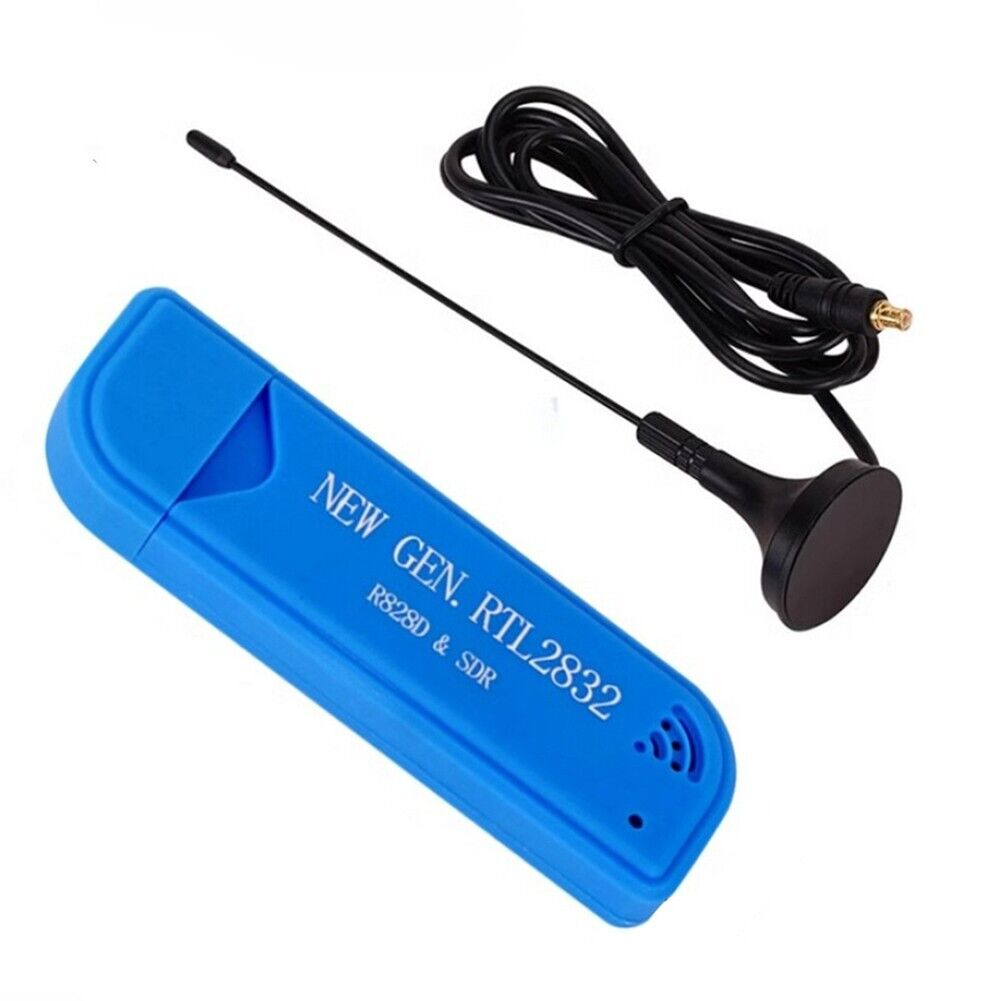
\includegraphics[width=0.3\textwidth]{rtlSdr.jpg}
    \caption{RTL-SDR with Simple SMA Antenna}
    \label{fig:rtlSDR}
\end{figure}

The RTL-SDR is based on the Realtek RTL2832U chipset, and has a frequency range of 24MHz to 1.7GHz, and a bandwidth of 3.2MHz. The RTL-SDR is also relatively cheap, with a price of around \$40 AUD, coming with compatibility to a wide range of software, including MATLAB, and GNU radio \cite{SDRdongle}. More specifically, the RTL-SDR was originally designed as a DVB-T receiver for digital TV, but due to its versatility, it has been repurposed by the hobbyist community for a wide range of RF signal reception applications. Fundamentally, the RTL-SDR is compised of two IC chips as seen in the block diagram figure below \ref*{fig:rtlSDRblock}; the RTL2832U, which is the digital TV demodulator, and the R820T, which is the tuner. The R820T is the chip that allows the RTL-SDR to tune to a wide range of frequencies, converting those signal frequencies to an intermediate baseband frequency which is processed by the RTL2832U. Inside the RTL2832U, the signal is then digitized and demodulated and sent to the host computer via USB.

\begin{figure}[htbp]
    \centering
    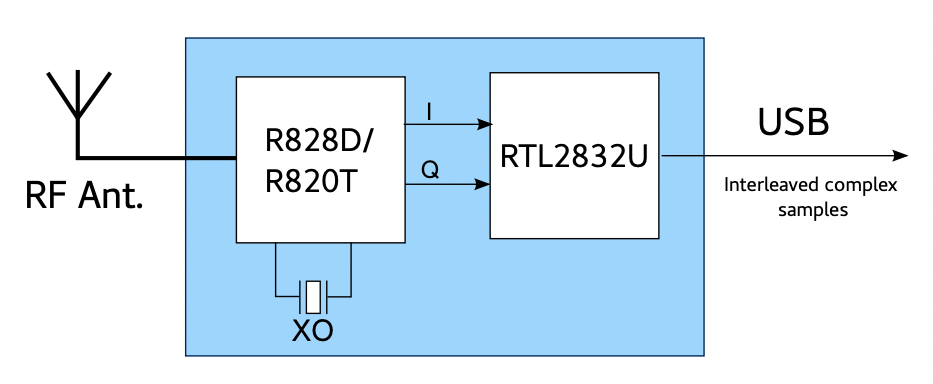
\includegraphics[width=0.7\textwidth]{rtlSDRchips.png}
    \caption{RTL-SDR Block Diagram \cite{RTLsdrBlockDiagram}}
    \label{fig:rtlSDRblock}
\end{figure}

\par \noindent
% NEEDS SPECIFIC TESTING STEPS

In order to test the functionality and performance of the RTL-SDR, it was necessary to perform the following steps in isolation before integrating into the testbeed, which are reflected in the results section:
% Testing steps
\begin{itemize}
    \item \textbf{Software Installation:} Install the RTL-SDR drivers and software on the relevant host computers (RPi5 and M1 Mac).
    \item \textbf{Signal Reception:} Tune the RTL-SDR to the appropriate frequency range (approx 200MHz) and receive a digital broadcast signal (with yagi-uda antenna or simple SMA monopole).
    \item \textbf{Signal Processing:} Process the received signal values using python to ensure the values are not junk.
    \item \textbf{Noise Floor Measurement:} Measure the noise floor of the received signal to account for the signal-to-noise ratio (SNR) of the system (given test location).
\end{itemize}

\vspace{0.5cm} \noindent 
\textbf{(ii) LimeSDR}
The LimeSDR was chosen as the higher end SDR module for the implementation and testing of the testbed. As seen in Table \ref{tab:SDRcomparison}, the LimeSDR has a frequency range of 100kHz to 3.8GHz, and a bandwidth of 61.44MHz. The LimeSDR is also more expensive than the RTL-SDR, with a price of around \$600 AUD. Specifically, the LimeSDR used was the LimeSDR-USB Version 1.4, which can be seen in the figure below \ref{fig:limeSDR}. 

\begin{figure}[htbp]
    \centering
    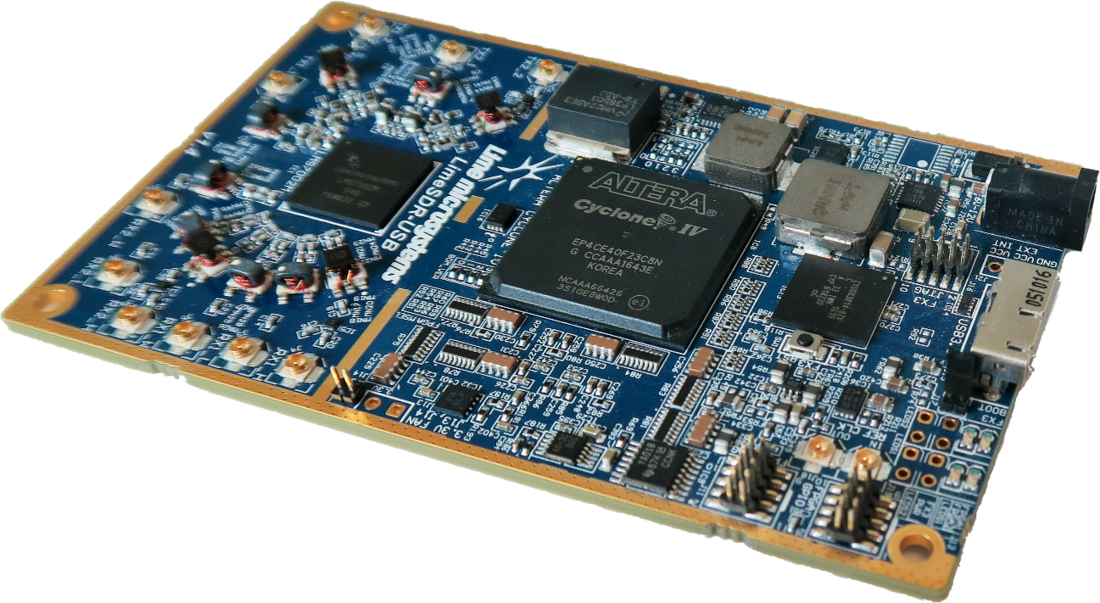
\includegraphics[width=0.3\textwidth]{limeSDR.png}
    \caption{LimeSDR-USB Version 1.4 PCB \cite{limesdr_usb}}
    \label{fig:limeSDR}
\end{figure}

The actual SDR module was encased as seen in XXX \ref{fig:finalTestbed}, with the only relevant conenctions being a singular RX SMA port, power supply (6V DC) and a USB type B connection. The block diagram of the LimeSDR can be seen in the figure below \ref{fig:limeSDRblock}, and evidently it is a more complex system than the RTL-SDR, most notably with the CycloneIV FPGA chip, which is used for signal processing and control.

In order to validate the standalone functionality of the LimeSDR, the following steps were taken, and discussed in the results section:
\begin{itemize}
    \item \textbf{Software Installation:} Install the LimeSDR drivers and software, the software required is in section \ref{sec:SDRsoftware}.
    \item \textbf{Signal Reception:} Tune the LimeSDR to the appropriate frequency range (approx 200MHz) and receive a digital broadcast signal (with yagi-uda antenna).
    \item \textbf{Signal Processing:} Process the received signal values using python to ensure the values are not junk.
    \item \textbf{Noise Floor Measurement:} Measure the noise floor for given location.
\end{itemize}

\begin{figure}[htbp]
    \centering
    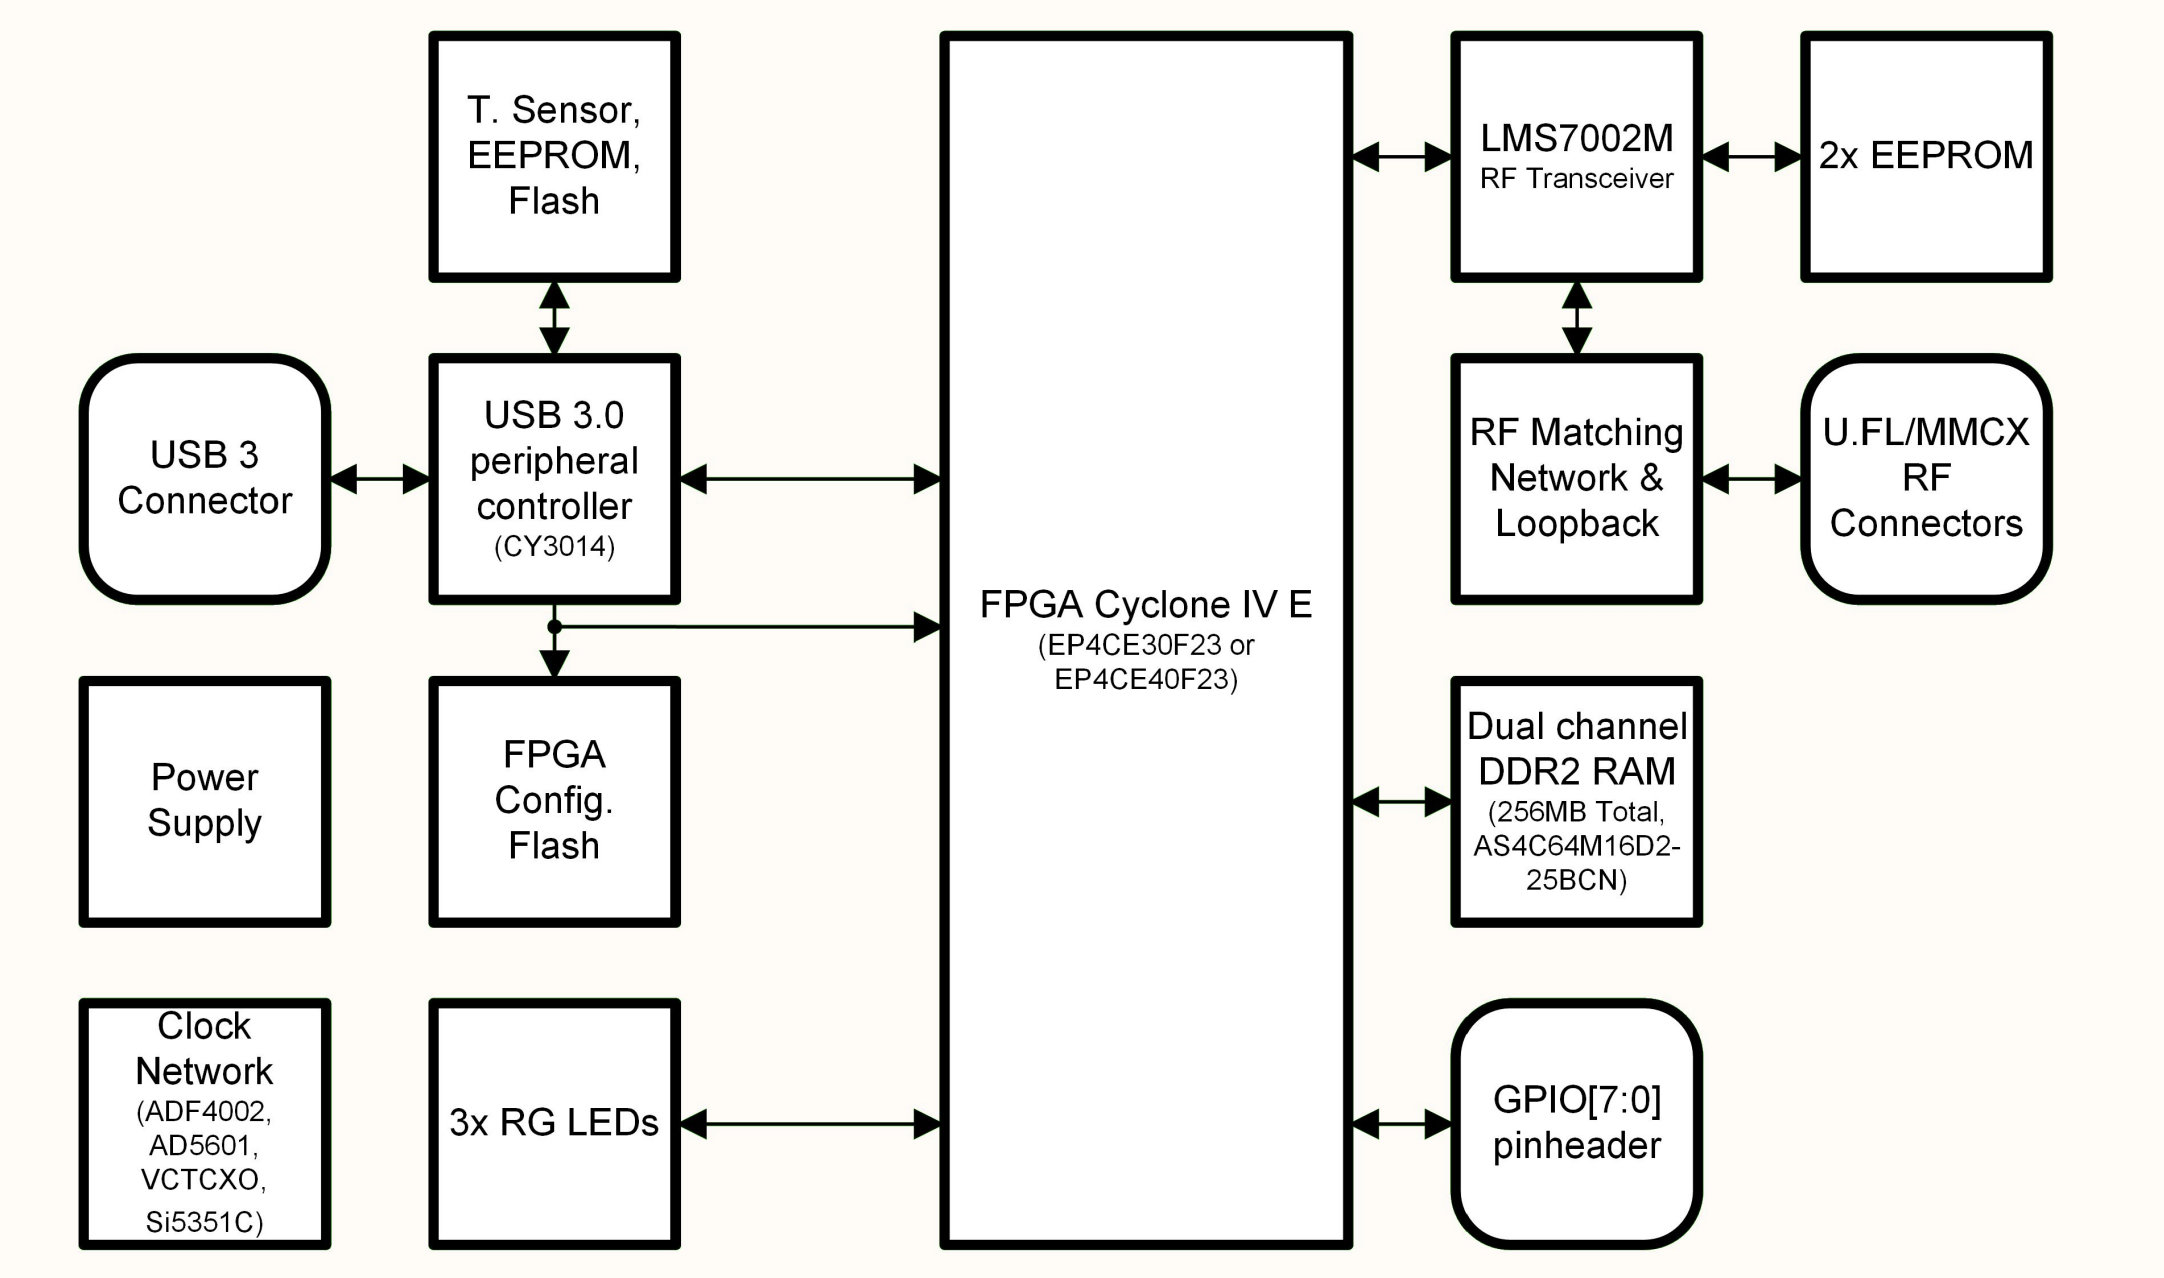
\includegraphics[width=0.7\textwidth]{limeSDRblock.png}
    \caption{LimeSDR Block Diagram \cite{limesdr_usb}}
    \label{fig:limeSDRblock}
\end{figure}

Another notable hardware feature of the LimeSDR is the LMS7002M transceiver chip which can facilitate both RX and TX capabilities, along with built in ADC/DAC (12 bit) capability \cite{limesdr_usb}. The bandwidth advantage of the LimeSDR was a key factor in its selection, as the wider bandwidth allows for more data to be captured and processed, specifically in the context of the digital broadcast signal used as the illuminator of opportunity. This bandwidth advantage directly results in increased range resolution on the range doppler maps, which is a key metric for the detection of aerial vehicles. As seen in \ref{tab:SDRcomparison}, the LimeSDR has a stated maximum sampling rate of 61.44MHz,, when sampling at this rate, the bottlneck can become the USB host interface. With the maximum sample rate corresponding to about 240MB/s, which if not over USB 3.0 can limit the data transfer rate (USB 2.0 is limited to 480Mbps or 60MB/s). Moreover, as the maximum sampling rate is approached, the storage and processing requirements of the host computer also increase, becoming unreasonable at a certain point for samples of around 10 seconds.

\subsection{Embedded Computing Platform \label{sec:embedded computing}}


The embedded computing platform chosen for the testbed was the Raspberry Pi 5 (RPi5), specifically the version with 8GB of RAM \cite{core_electronics_rpi5}. 

\begin{figure}[htbp]
    \centering
    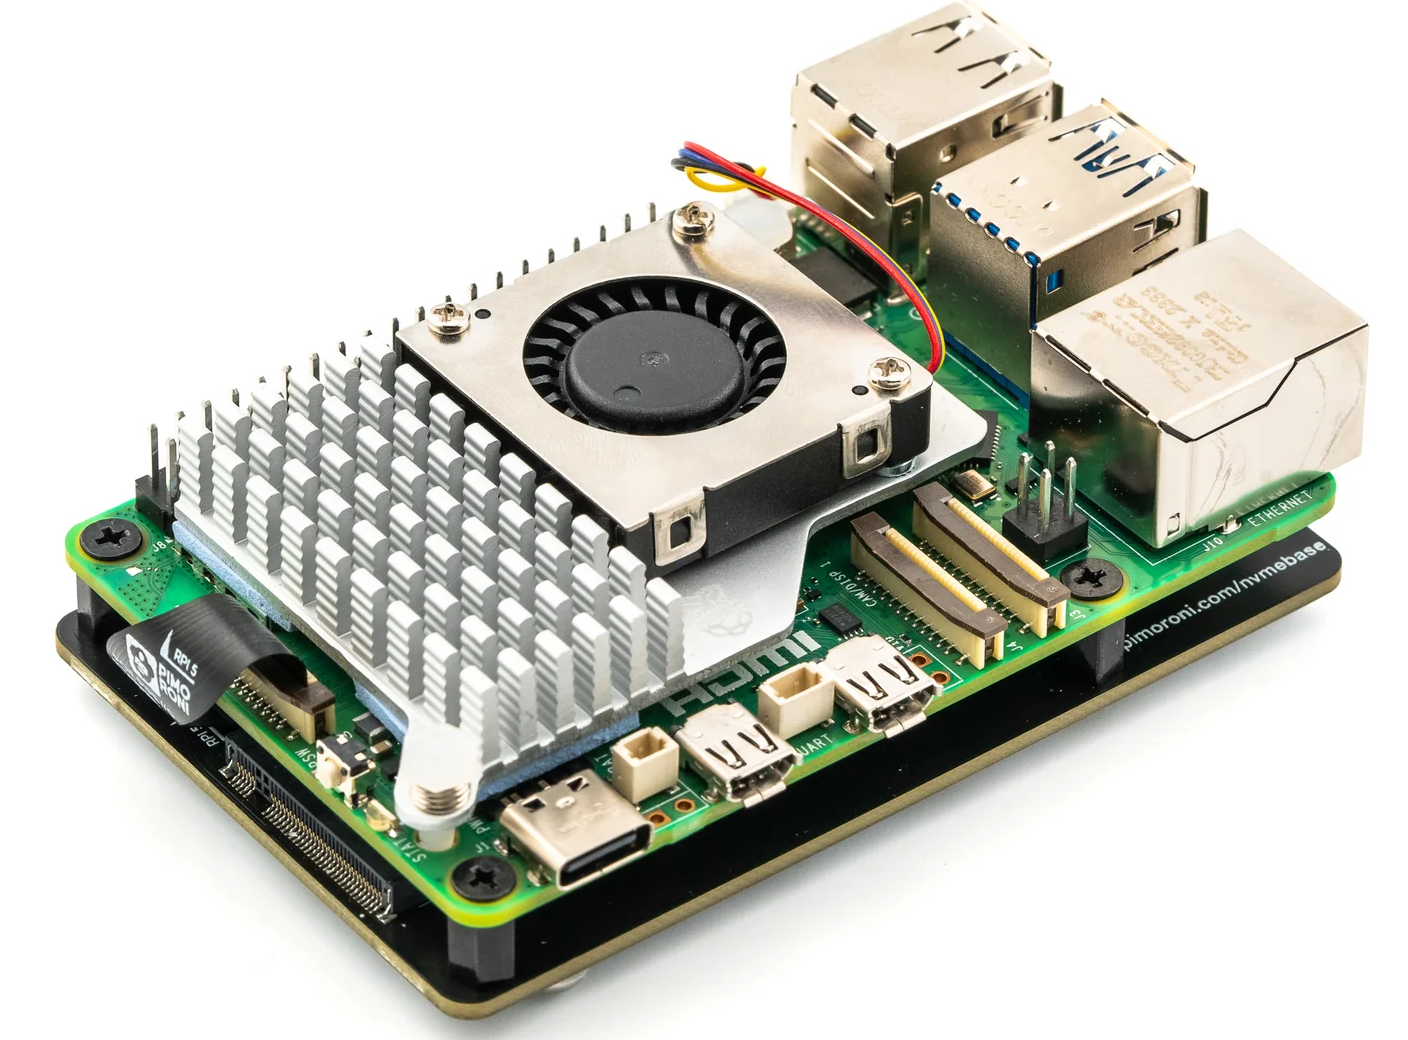
\includegraphics[width=0.3\textwidth]{nvmeRpi5.png}
    \caption{Raspberry Pi 5 with NVME SSD \cite{pimoroni_nvme_base}}
    \label{fig:Rpi5}
\end{figure}

As seen in Table \ref{tab:sbc_comparison}, the RPi5 has a quad-core ARM Cortex-A72 CPU, 8GB of LPDDR4-3200 SDRAM, and a 1Gbit Ethernet port. The RPi5 was chosen for its relatively low cost, small form factor, and wide range of software support. Other SBC's from Table \ref{tab:sbc_comparison} were considered, but the Rpi5 represented the best balance of performance and cost for the project, for example, the higher cost of the Nvidia Jetson was not justified for the project requirements. The viability of the Raspberry Pi5 in the context of testbed design and functionality was analysed based on the following points:

\noindent \textbf{Advantages}
\begin{itemize}
    \item \textbf{Storage:} The RPi5 supports external storage options via microSD, along with configurable HATs (hardware attached on top) for NVME SSDs, see section \ref{sec:storage} \cite{pimoroni_nvme_base}.
    \item \textbf{Size:} Its small form factor (85.6 x 56.5 mm) - roughly the size of a credit card, makes it easy to integrate into a testbed setup. Easily obtainable cooling fan.
    \item \textbf{GPIO:} 40 Pin GPIO header, can be used for interfacing with a prospective testbed user. Driven by the RP1 (custom I/O controller chip) \cite{core_electronics_rpi5}, the I/O is programmable with python.
    \item \textbf{Networking Capability:} Includes a 1Gbit Ethernet port and Wi-Fi 802.11ac, facilitating high-speed data transfer and network communication. Capable of 217.6 MB/s over Wi-Fi \cite{rpi5_wifi}.
    \item \textbf{Processing Capability:} Equipped with a quad-core ARM Cortex-A72 CPU and 8GB of LPDDR4-3200 RAM, enabling 2.4 GHz clock \cite{core_electronics_rpi5}.
    \item \textbf{Cost-Effectiveness:} Price of \$150 AUD, making it an affordable option for the project, approximately 1.5 the cost of the RPi4 (however almost double the performance) \cite{core_electronics_rpi5}
    \item \textbf{Software Support:} Extensive community support and availability of a wide range of software tools and libraries, especially for Linux-based systems, e.g. RTL-SDR, GNU Radio, etc. see section \ref{sec:SDRsoftware}.
\end{itemize}

\noindent \textbf{Disadvantages}
\begin{itemize}
    \item \textbf{Limited Built-In Storage:} The built-in storage is minimal, so additional external storage is necessary for handling large volumes of data.
    \item \textbf{Performance Constraints:} While powerful, it may not handle very high-frequency or complex radar signal processing as efficiently as more specialized or high-performance computing platforms, custom algorithms potentially required \cite{IOTpassiveRadar}.
    \item \textbf{Heat Management:} Under continuous heavy load, the RPi5 may require additional cooling solutions to prevent overheating.
    \item \textbf{Limited I/O Bandwidth:} The available I/O bandwidth might be a bottleneck for applications requiring very high-speed data acquisition and processing.
    \item \textbf{Power Supply:} Requires a stable power supply of 5.1V / 15W; not ideal for potentially portable or battery-powered applications \cite{rpi5_wifi}. 
\end{itemize}



\subsection{NVME Based Storage \label{sec:storage}}
Following on from the selection and testing of the Raspberry Pi 5 as the testbed computing platform, it became evident that the default 32GB microSD card used to boot and run the operating system was insufficient for the storage requirements of the project. The chosen solution for the bottleneck was to utilise a NVME SSD drive, connected via PCIe to the Raspberry Pi 5, specifically the Pimoroni Base \cite{pimoroni_nvme_base}. It was necessary to test the efficacy of the NVME SSD in the context of the testbed, with the following steps take and discussed in the results section:
% Steps for testing the NVME SSD
\begin{itemize}
    \item \textbf{Hardware Installation:} Screw the NVME SSD drive into the Pimoroni Base, and connect the Base to the Raspberry Pi 5 via the PCIe connector.
    \item \textbf{Software Configuration:} Format the NVME SSD drive with operating system.
    \item \textbf{Performance Testing:} Test the read and write performance of the NVME SSD drive using the \texttt{hdparm} utility.
\end{itemize}

Further NVME SSD configuration details include formatting with the ext4 file system, which is the default for most Linux distributions. It was mounted to the Raspberry Pi 5 (RPi5) at the location /mnt/nvme0n1. The SSD connects via a PCIe x4 interface Gen 2.0, a high-speed standard commonly used for storage devices. It supports M.2 NVMe drives of the 2280 size. The specific model used is the Patriot P300 NVMe M.2 SSD with a 128GB capacity, serving both as storage and for booting the RPi5.


\subsection{Antenna Configuration \label{sec:antenna}}
Intially, a simple SMA whip antenna was used for the RTL-SDR, as seen in Figure \ref{fig:rtlSDR}. These low cost antennas are typically used for general purpose reception, and are not optimised for any specific frequency range. The whip antenna was used for initial testing and prototyping, and was capable of receiving a range of broadcast signals with a NOISE FLOOR X. Eventually a more specialised antenna was used, the Yagi-Uda antenna, which is a directional antenna that is commonly used for point-to-point communication. The Yagi-Uda antenna was used for the final testing and validation of the testbed. The Yagi-Uda was utilised with a CLF200 50 Ohm coaxial cable, which was connected to the RTL-SDR. Specifically, the 18 element UHF yagi-uda antenna, was quoted as having 15.5dB forward gain and 25dBi front-to-back ratio \cite{AntennaPiece}. Typically, with directional antennas, such as the Yagi-Uda, when the gain is increased, the beamwidth is decreased, which is ideal for the testbed setup, as the antenna was placed in a specific location to receive the illuminator signal.

The physical setup of these antennas for testing comprised of an "Over the Shoulder" geometry whereby the antenna was placed behind a building in the line of sight of the TX signal (in this case Mt Cootha). For a single channel / antenna PBR setup, this geometry works to attenuate the direct path signal, and allow for the reflection to be better received by the antenna. The resulting attenuation of the direct signal from the geometry can be estimated around \textbf{ -10dB} based on previous studies \cite{GeometryAttenuation}.


\begin{figure}[htbp]
    \centering
    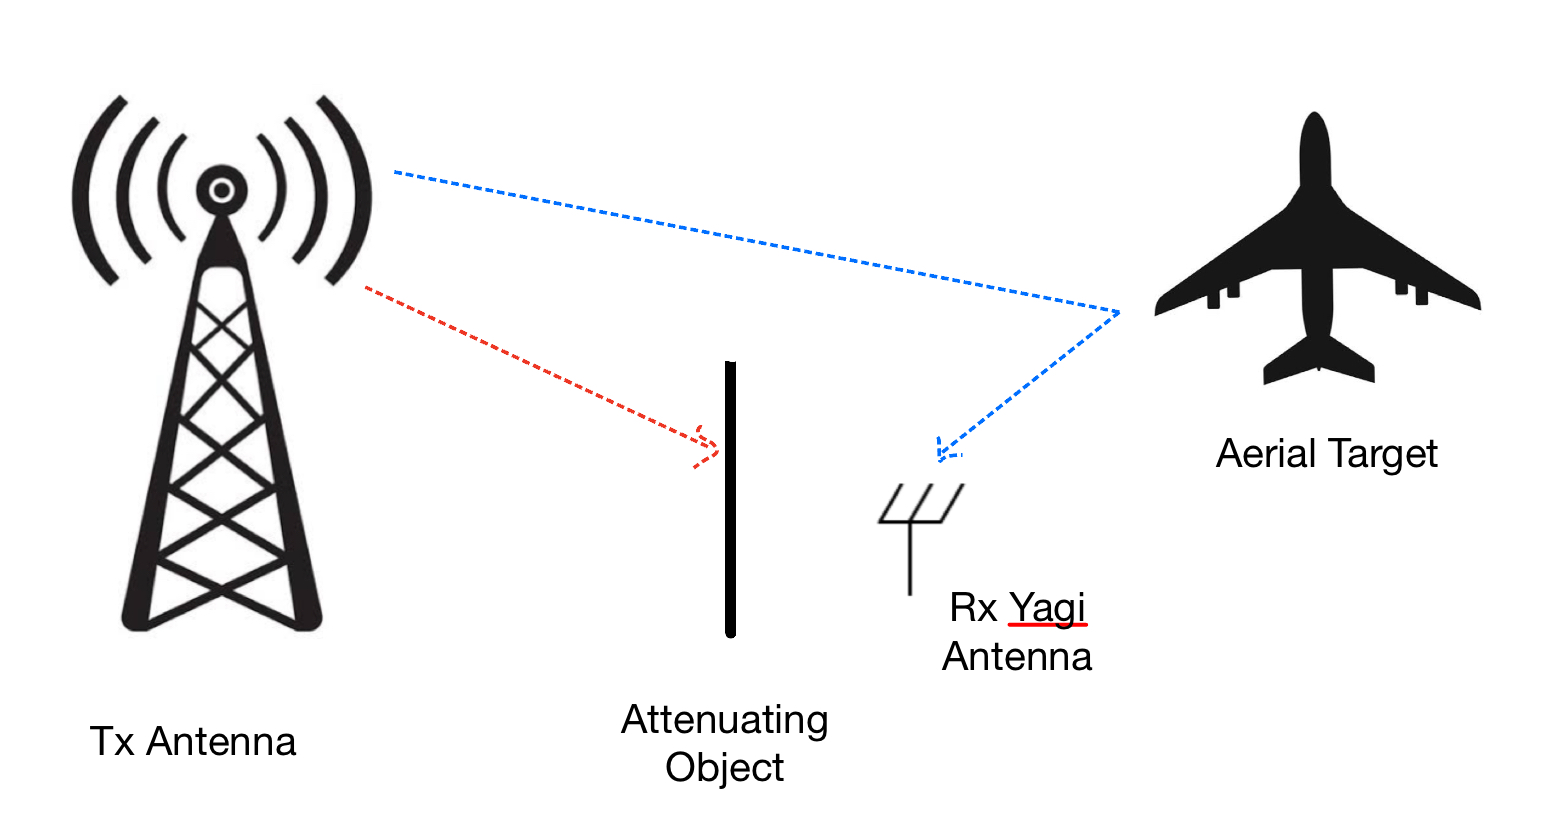
\includegraphics[width=0.8\textwidth]{overShoulder.png}
    \caption{Geometry of Over the Shoulder Antenna Placement}
    \label{fig:overTheShoulder}
\end{figure}



\subsubsection{Antenna Verification and Testing Requirements}
It was necessary to have a range of hardware verification tests to ensure the antenna was functioning correctly and to quantify the signal strength of the illuminator signal. The following steps were taken to test the signal strength of the illuminator signal, and are discussed in the results section:
\begin{itemize}
    \item \textbf{Signal Strength Measurement:} Measure the signal strength of the illuminator signal using the RTL-SDR and the SMA whip antenna.
    \item \textbf{Signal Strength Comparison:} Compare the signal strength of the illuminator signal using the RTL-SDR and the Yagi-Uda antenna.
    \item \textbf{Compare a Range of Test Locations:} Given the geography of Mt Cootha and the Brisbane air traffic fligh path (INSERT RELEVANT GEOGRAPHY MAP), it was necessary to test the signal strength at a range of locations to ensure the illuminator signal was being received, and compare any contributable noise factors.
\end{itemize}


\subsection{Testbed Design \label{sec:testbed}}
Building off the aforementioned hardware components, it was then necessary to develop a physical testbed setup that would allow for the SDR receiver module to be connected to the embedded computing platform, and for the entire system to be powered and networked. Also, given the scope of the project, it was necessary to have a protective encasing for the Rpi5 which also implemented user functionality (ie. pushbuttons and LED's). The testbed was designed to be portable and easily deployable, with the following key components and features:

\begin{itemize}
    \item \textbf{Enclosure:} A custom 3D printed enclosure was designed to house the RPi5, the RTL-SDR, and the NVME SSD HAT seen in \ref{fig:Rpi5}. The enclosure was designed to be compact and portable, with a small form factor that could be easily transported and deployed in various environments. The enclosure was designed to be easily opened and closed, with a removable top panel that allowed for easy access to the internal components. The printed acrylic was also designed for cooling purposes, with ventilation holes on the top and sides of the enclosure to allow for airflow, bolstered by the Rpi5 active cooling fan and heatsink. The model from Rasmussen was identified as a base model, with potential for appropriate modification \cite{RPiCase}. 
    \item \textbf{User Interface:} It was envisaged that the testbed have some sort of capability that would enable physical triggering of PBR sampling and processing. Arcade style pushbuttons with LED's were selected to facilitate this interface \cite{pushbuttons}. It was envisaged that one pushbutton be responsible for signal sampling and the other a trigger for embedded edge processing. 
    \item \textbf{Power Supply:} A 5V / 15W power supply was used to power the RPi5, with a USB-C connector that allowed for easy connection to the RPi5. 
    \item \textbf{Networking:} The ethernet port on the Rpi5 was left unobstructed by the case for potential wired networking. With the main focus of being geared towards Wi-Fi based networking which was all facilitated by the Rpi5 system on chip.
    \item \textbf{Radio Front End:} It was intended for the SDR module to be connected via the USB 3.0 port with the enclosure not designed to house the SDR unit (for versatility). Per SDR functionality, the antenna was connected via coaxial cable, also not housed in the enclosure. 
    
\end{itemize}

In summary, the testbed was designed to be a portable, easily deployable system that could be used to test and validate the passive radar detection system. The enclosure was designed to house the RPi5, the NVME HAT, with the remaining system hardware components not specific to the testbed itself (possible to change out). This part of the project design was important for achieving the primary objectives, notably objective 2 as stated in \ref{sec:aims}. Details of the actual build process and testing of the enclosure are discussed in \ref{sec:enclosureResults}.

\section{Software}

\subsection{SDR Software \label{sec:SDRsoftware}}
When utilising SDR modules, it is necessary to have capabilities to perform necessary processing on the sampeld data. This is typically done using SDR 'driver' software, which is a type of software that allows for the reception and baseband processing of radio signals using SDR hardware (ie. setting the tuner to a given frequency). Both the SDR modules utilised communicated with the host computer via USB 3.0, and utilise the libusb library for this. In the case of the selected hardware for this project, it was necessary to utilise relevant driver API's to interface with the RTL-SDR and LimeSDR, both from the testbed and the higher level M1 Mac, as shown below.

\vspace{0.5cm} \noindent 
\textbf{(i) RTL-SDR} Given the widespread use of RTL-SDR dongles, there is a range of useable software stacks and drivers available. The interface software utilised for testing and visualising the RTL-SDR efficacy was GQRX, which is a software defined radio receiver powered by GNU Radio and the Qt GUI toolkit. GQRX is easy to use and provides a range of features for signal processing and analysis \cite{RTLSDRchipSet}. The software was installed on the RPi5 and the M1 Mac, and was used to receive and process the digital broadcast signal, also helping test the antenna. Whilst GQRX is used as a front end visualisation tool, it essentially wraps the \textbf{librtlsdr} library \cite{librtlsdr}, which is the actual API driver for the RTL-SDR (specifically the RTL2832U chip \cite{RTLSDRspecs}). The librtlsdr library handles hardware communication, tuning, and data acquisition (gain, sampling, etc) \cite{librtlsdr}, and consequently outputs 8-bit I/Q samples to the host computer. This library was tested on both the RPi5 and the M1 Mac, as seen in the results section.

\vspace{0.5cm} \noindent 
\textbf{(ii) LimeSDR} The LimeSDR requires a more complex software stack than the RTL-SDR, given its higher performance and comparitively better hardware. As mentioned in section \ref{sec: SDRdongleHardware} and specifically seen in the LimeSDR block diagram \ref{fig:limeSDRblock}, the LimeSDR has a custom LMS7002M transceiver chip, along with other programmable components. However, given the relatively smaller user numbers of the LimeSDR it was more difficult to interface (given lack of documentation). The following software was used to interface with the LimeSDR, the connection between these APIs can be viewed in the software block diagram below \ref{fig:limeSDRapi}:

% software api block diagram
\begin{figure}[htbp]
    \centering
    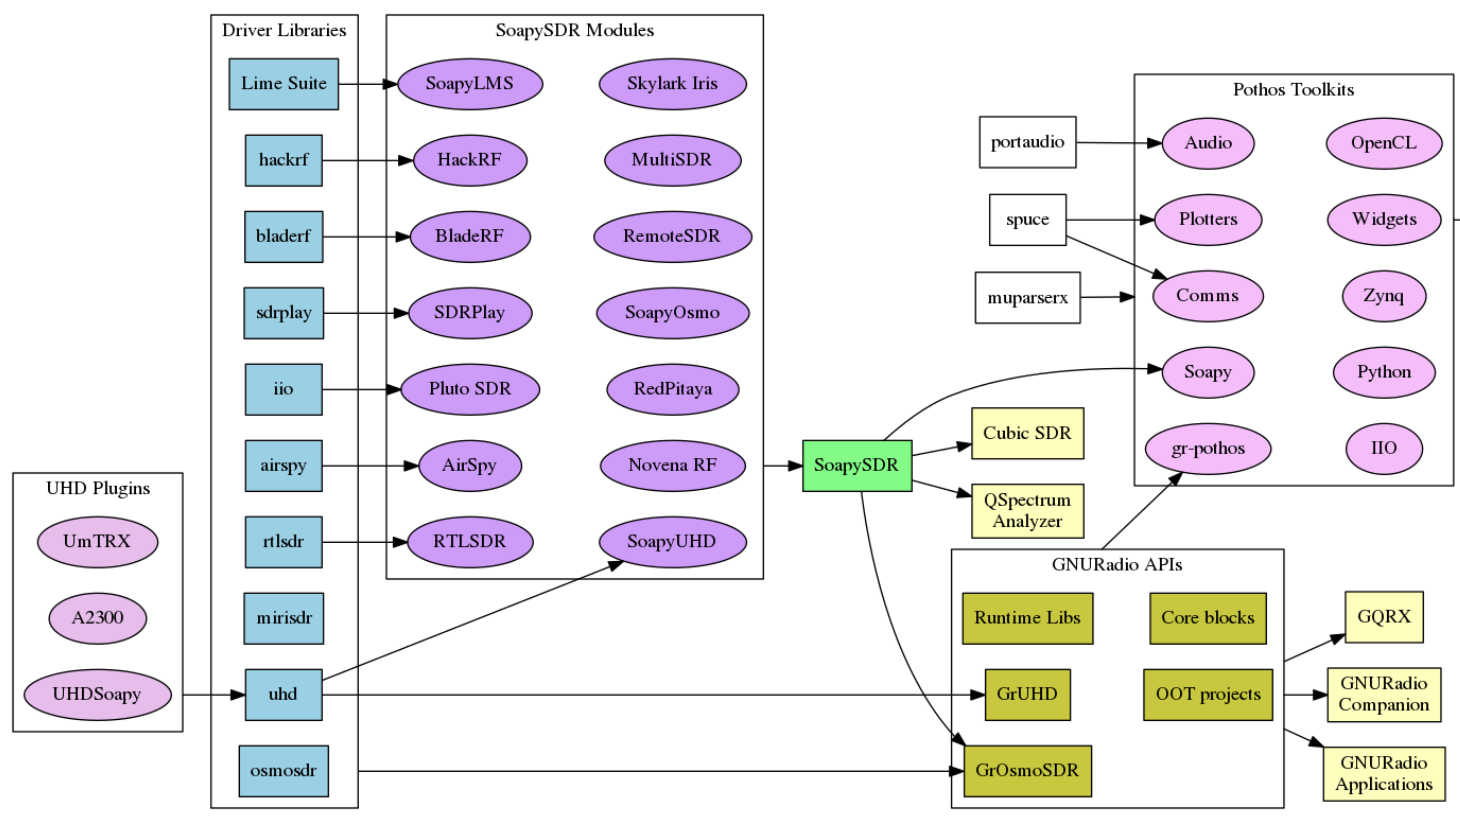
\includegraphics[width=0.78\textwidth]{APIframework.png}
    \caption{LimeSDR Software API Block Diagram}
    \label{fig:limeSDRapi}
\end{figure}

\begin{itemize}
    \item \textbf{LimeSuite:} LimeSuite is the software that is used to interface with the LimeSDR hardware, and is used to configure the LimeSDR, set the frequency, gain, and bandwidth, and perform other functions \cite{limesdr_usb}. 
    \item \textbf{SoapySDR:} SoapySDR \cite{soapsdr} is a software abstraction layer that provides a common API for interfacing with a wide range of SDR hardware, including the LimeSDR. SoapySDR provides a simple and consistent API for interfacing with SDR hardware, and is used to communicate with the LimeSDR hardware from the host computer \cite{soapsdr}. It essentially acts to wrap and unify the LimeSuite and LimeSDR hardware, providing a common interface for the host computer (ideal for porting from testbed to high level mac)
    \item \textbf{Python:} Python was used as an abstract interface, essentially calling the SoapySDR API, again, easily transferable between host computers. 
\end{itemize}

In summary, the above software was selected to ensure portability between both the testbed and the higher level M1 Mac, whilst also accounting for potential SDR hardware changes. The individual component testing comprised of sampling DAB 9A, ensuring correct file parsing and basic noise floor readings.

\subsection{Networking Requirements \label{sec:networking}}
Given the abundance of options explored in the background section, initially, the Raspberry Pi was connected to via SSH and VNC viewer over WiFi for configuration and testing. Eventually TCP baswed client-server communication was used to facilitate the transfer of data between the RPi5 and the M1 Mac. The TCP server was implemented in Python on the M1 Mac, and the TCP client was implemented in Python on the M1 Mac. The TCP client was responsible for sending the sampled data to the TCP client, which was responsible for receiving the data and processing it. This was implemented via the \texttt{socket} library in Python, and was tested on the RPi5 and the M1 Mac, with the results discussed in the results section.


% METHOD FOR TESTING Comparison
\section{Relevant Digital Signal Processing}

Once the first phase of the testbed verification was completed, the next step was to implement the digital signal processing (DSP) algorithms that would be used to process the received signals and detect the presence of aerial vehicles, and then compare the results between the RTL-SDR and the LimeSDR, along with edge compute times (on the Rpi5) and higher level mac processing. Whilst both SDR implementations used the same fundamental DSP algorithms (FFT and autocorrelate), there were some system factors that were impacted by the comparison. A high level overview of the processing chain can be seen in the block diagram below \ref{fig:processingChain}:

\begin{figure}[htbp]
    \centering
    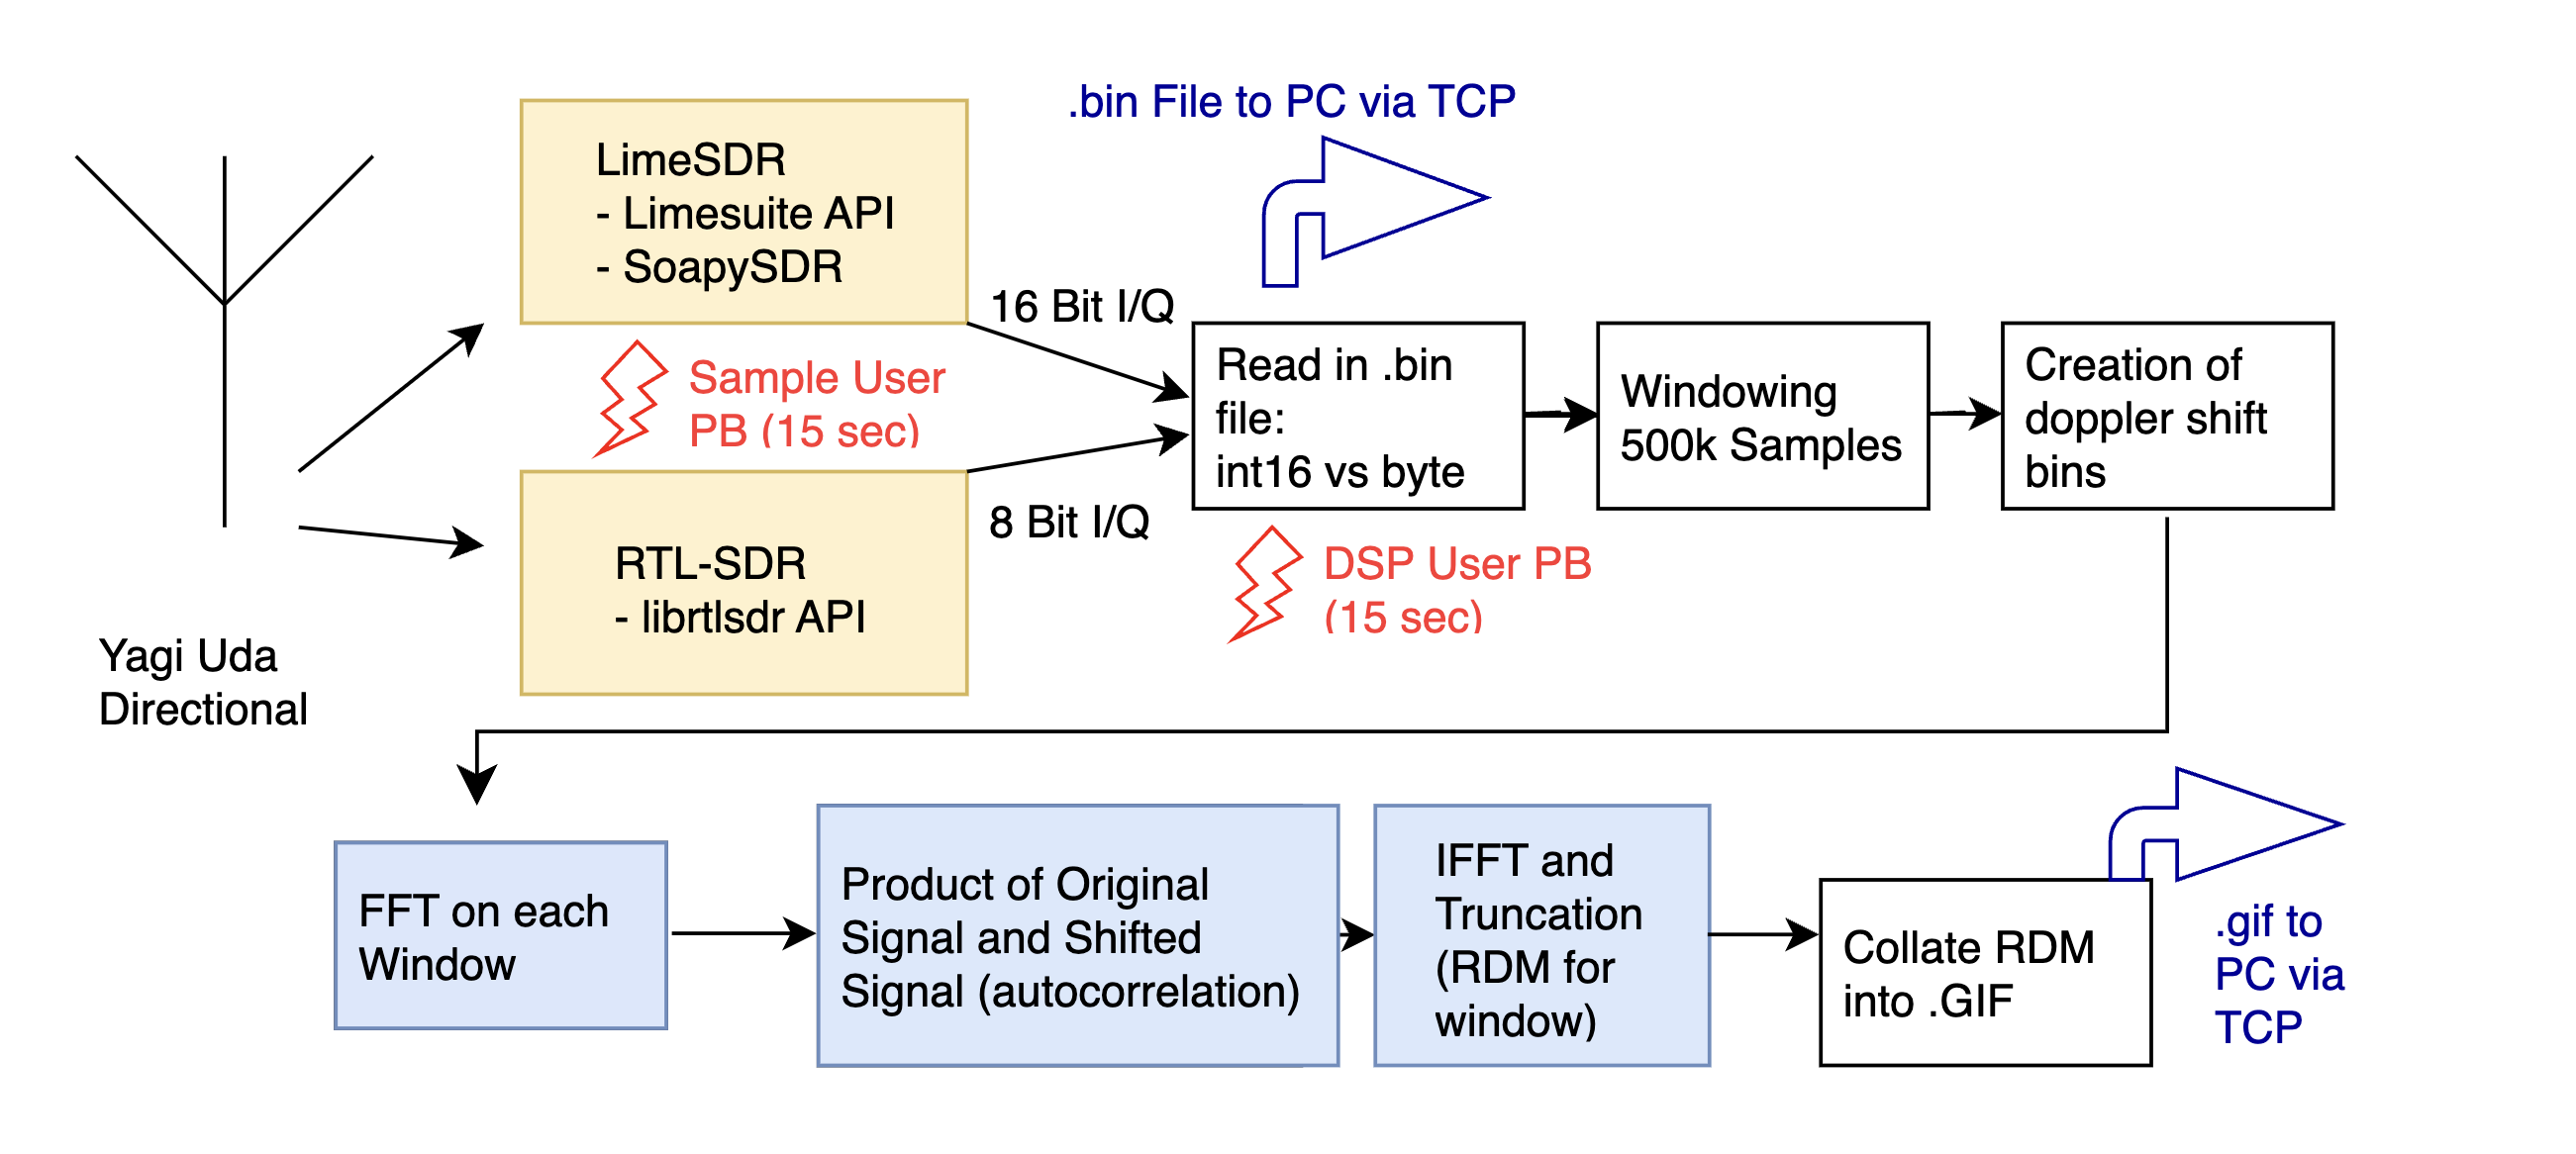
\includegraphics[width=0.8\textwidth]{SystemFlow.png}
    \caption{Digital Signal Processing Chain}
    \label{fig:processingChain}
\end{figure}

Based on the windowing of \textbf{500k} samples, the theoretical maximum detection range of the system can be calculated. Given a default sample rate of 2.048MHz, the range resolution is calculated as follows: 

\[
R_{\text{max}} = \frac{c \times N}{2 \times f_s}
\]

\[
R_{\text{max}} = \frac{3 \times 10^8 \, \text{m/s} \times 500,000}{2 \times 2.048 \times 10^6 \, \text{Hz}}
\]

\[
R_{\text{max}} \approx \frac{1.5 \times 10^{14}}{4.096 \times 10^6} \approx 36.6 \, \text{km}
\]

Thus, the theoretical maximum detection range is approximately \( 36.6 \, \text{km} \). However, this is a theoretical maximum, and without the use of filtering and clutter supression, the actual detection range will be much less. Furthemore, the actual detection range is also influenced by factors such as TX/RX geometry along with the other geographical factors \cite{DTSO2009}. The actual range, known as the dynamic range, is dependent on on relative position of receiver, target and transmitter as shown by Hughes in \ref{fig:geometry} \cite{FundamentalsPassiveRadar}.



\subsection{Selection of Illuminator Signal}
The illuminator of opportunity primarily explored for this project is the DAB+ signal, and the target signal will be aerial vehicles - most likely in the form of civillian passenger jets. The DAB+ signal is a good option due to its high power density, and its relatively high bandwidth, which can be used to improve the radar's resolution and ability to distinguish between targets and clutter. Moreover, the geographical proximity of a DAB+ transmitter at Mt Cootha to the University of Queensland, St Lucia campus, making it a potentially ideal choice for the project. Another prospective digital illuminator signal is DVB-T (digital video broadcast - terrestrial), which is similar in its digital modulation to DAB, but provides increased bandwidth and signal power \cite{DVBsignal}.

\subsection{Sampling Rate and Bandwidth}
Fundamentally, the LimeSDR supports much higher sampling rates and bandwidths than the RTL-SDR, with the LimeSDR having a maximum sampling rate of 61.44MHz compared to the RTL-SDR which has a maximum sampling rate of 3.2MHz. This difference in sampling rate and bandwidth has a direct impact on the range resolution of the radar system, with the LimeSDR being able to achieve much better range resolution than the RTL-SDR. The range resolution is dictated by the sampling rate (therefore bandwidth) according to the below:

\[
\Delta R = \frac{c}{2B}
\]

where:
\begin{itemize}
    \item \( \Delta R \): Range resolution (meters)
    \item \( c \): Speed of light (\(3 \times 10^8 \, \text{m/s}\))
    \item \( B \): Signal bandwidth (Hz) - DAB 1.536 MHz, DVB-T 7.5 MHz
\end{itemize}

The sampling rate and bandwidth of the SDR modules were tested and compared, with the results discussed in the results section. Based on the above equation, when sampling with a DVB-T signal / higher sampling rate the range resolution is improved, which is a key metric for the detection of aerial vehicles. The range resolution for each illuminator was:

\begin{itemize}
    \item \textbf{DAB+ Signal:} \( \Delta R = \frac{3 \times 10^8}{2 \times 1.536 \times 10^6} = 97.65625 \, \text{meters}\) - with IQ oversampling of 2.048Mhz, the range resolution is 73.2m.
    \item \textbf{DVB-T Signal:} \( \Delta R = \frac{3 \times 10^8}{2 \times 7.5 \times 10^6} = 20 \, \text{meters}\)
\end{itemize}

\subsection{Method for Testing and Comparing LimeSDR and RTL-SDR}
Both SDRs were connected to the RPi5 testbed and were used to receive the same digital broadcast signal. The received signals were then processed using the same DSP algorithms, and the results were compared. The following steps were taken to test and compare the LimeSDR and RTL-SDR:

\begin{itemize} 
    \item \textbf{RTL-SDR} Utilise the RTL-SDR to sample DAB+ 9A, in the algorithm, as seen in the block diagram \ref{fig:processingChain}, the fmap step size was varied to determine the optimal range resolution.
    \item \textbf{LimeSDR} Centered around DAB multiplex 9A, a range of sampling frequencies were applied: 2000MHz, 4000MHz, 80000Mhz - and then also experiment with a DVB-T signal of 177.5Mhz (channel 7 Brisbane). It is assumed that the DVB-T signal will provide a better range resolution, and thus better target detection.
\end{itemize}



